\newpage
\subsection{Diagramas de casos de uso}

Un diagrama de casos de uso es una representación visual perteneciente al lenguaje de modelado UML \textit{(Unified Modeling Language)} que describe las interacciones entre los actores del sistema y las funcionalidades que este ofrece. Su propósito es comunicar, de forma clara y estructurada, qué puede hacer el sistema y quién puede hacerlo, sin entrar en detalles de implementación. Cada caso de uso representa una funcionalidad específica que aporta valor al actor que la ejecuta, y las relaciones entre casos de uso permiten expresar dependencias obligatorias mediante \textit{ <<include>>} o comportamientos opcionales mediante \textit{<<extend>>}.

Dado que el sistema se compone de dos subsistemas complementarios, se presentan cuatro tipos de nomenclatura de etiquetado de casos de uso:

\begin{itemize}
    \item \textbf{CU-GX — General}: permite identificar los elementos compartidos entre la app móvil y la plataforma web.
    \item \textbf{CU-MX — App móvil}: detalla las funcionalidades disponibles para el actor Experto en la aplicación Android, abarcando desde el inicio de sesión hasta el flujo completo de captura, análisis y sincronización de registros en campo.
    \item \textbf{CU-WX —Plataforma web}: detalla las funcionalidades disponibles para el actor Experto en la plataforma web, orientada al monitoreo histórico del arbolado, la gestión de registros y la generación de reportes.
    \item \textbf{CU-AX — Administración}: detalla las funcionalidades exclusivas del actor Administrador dentro de la plataforma web, incluyendo la gestión de usuarios.
\end{itemize}

A continuación se presentan los diagramas de casos de uso que conforman el modelo de interacción del sistema.

\begin{figure}[H]
    \centering
    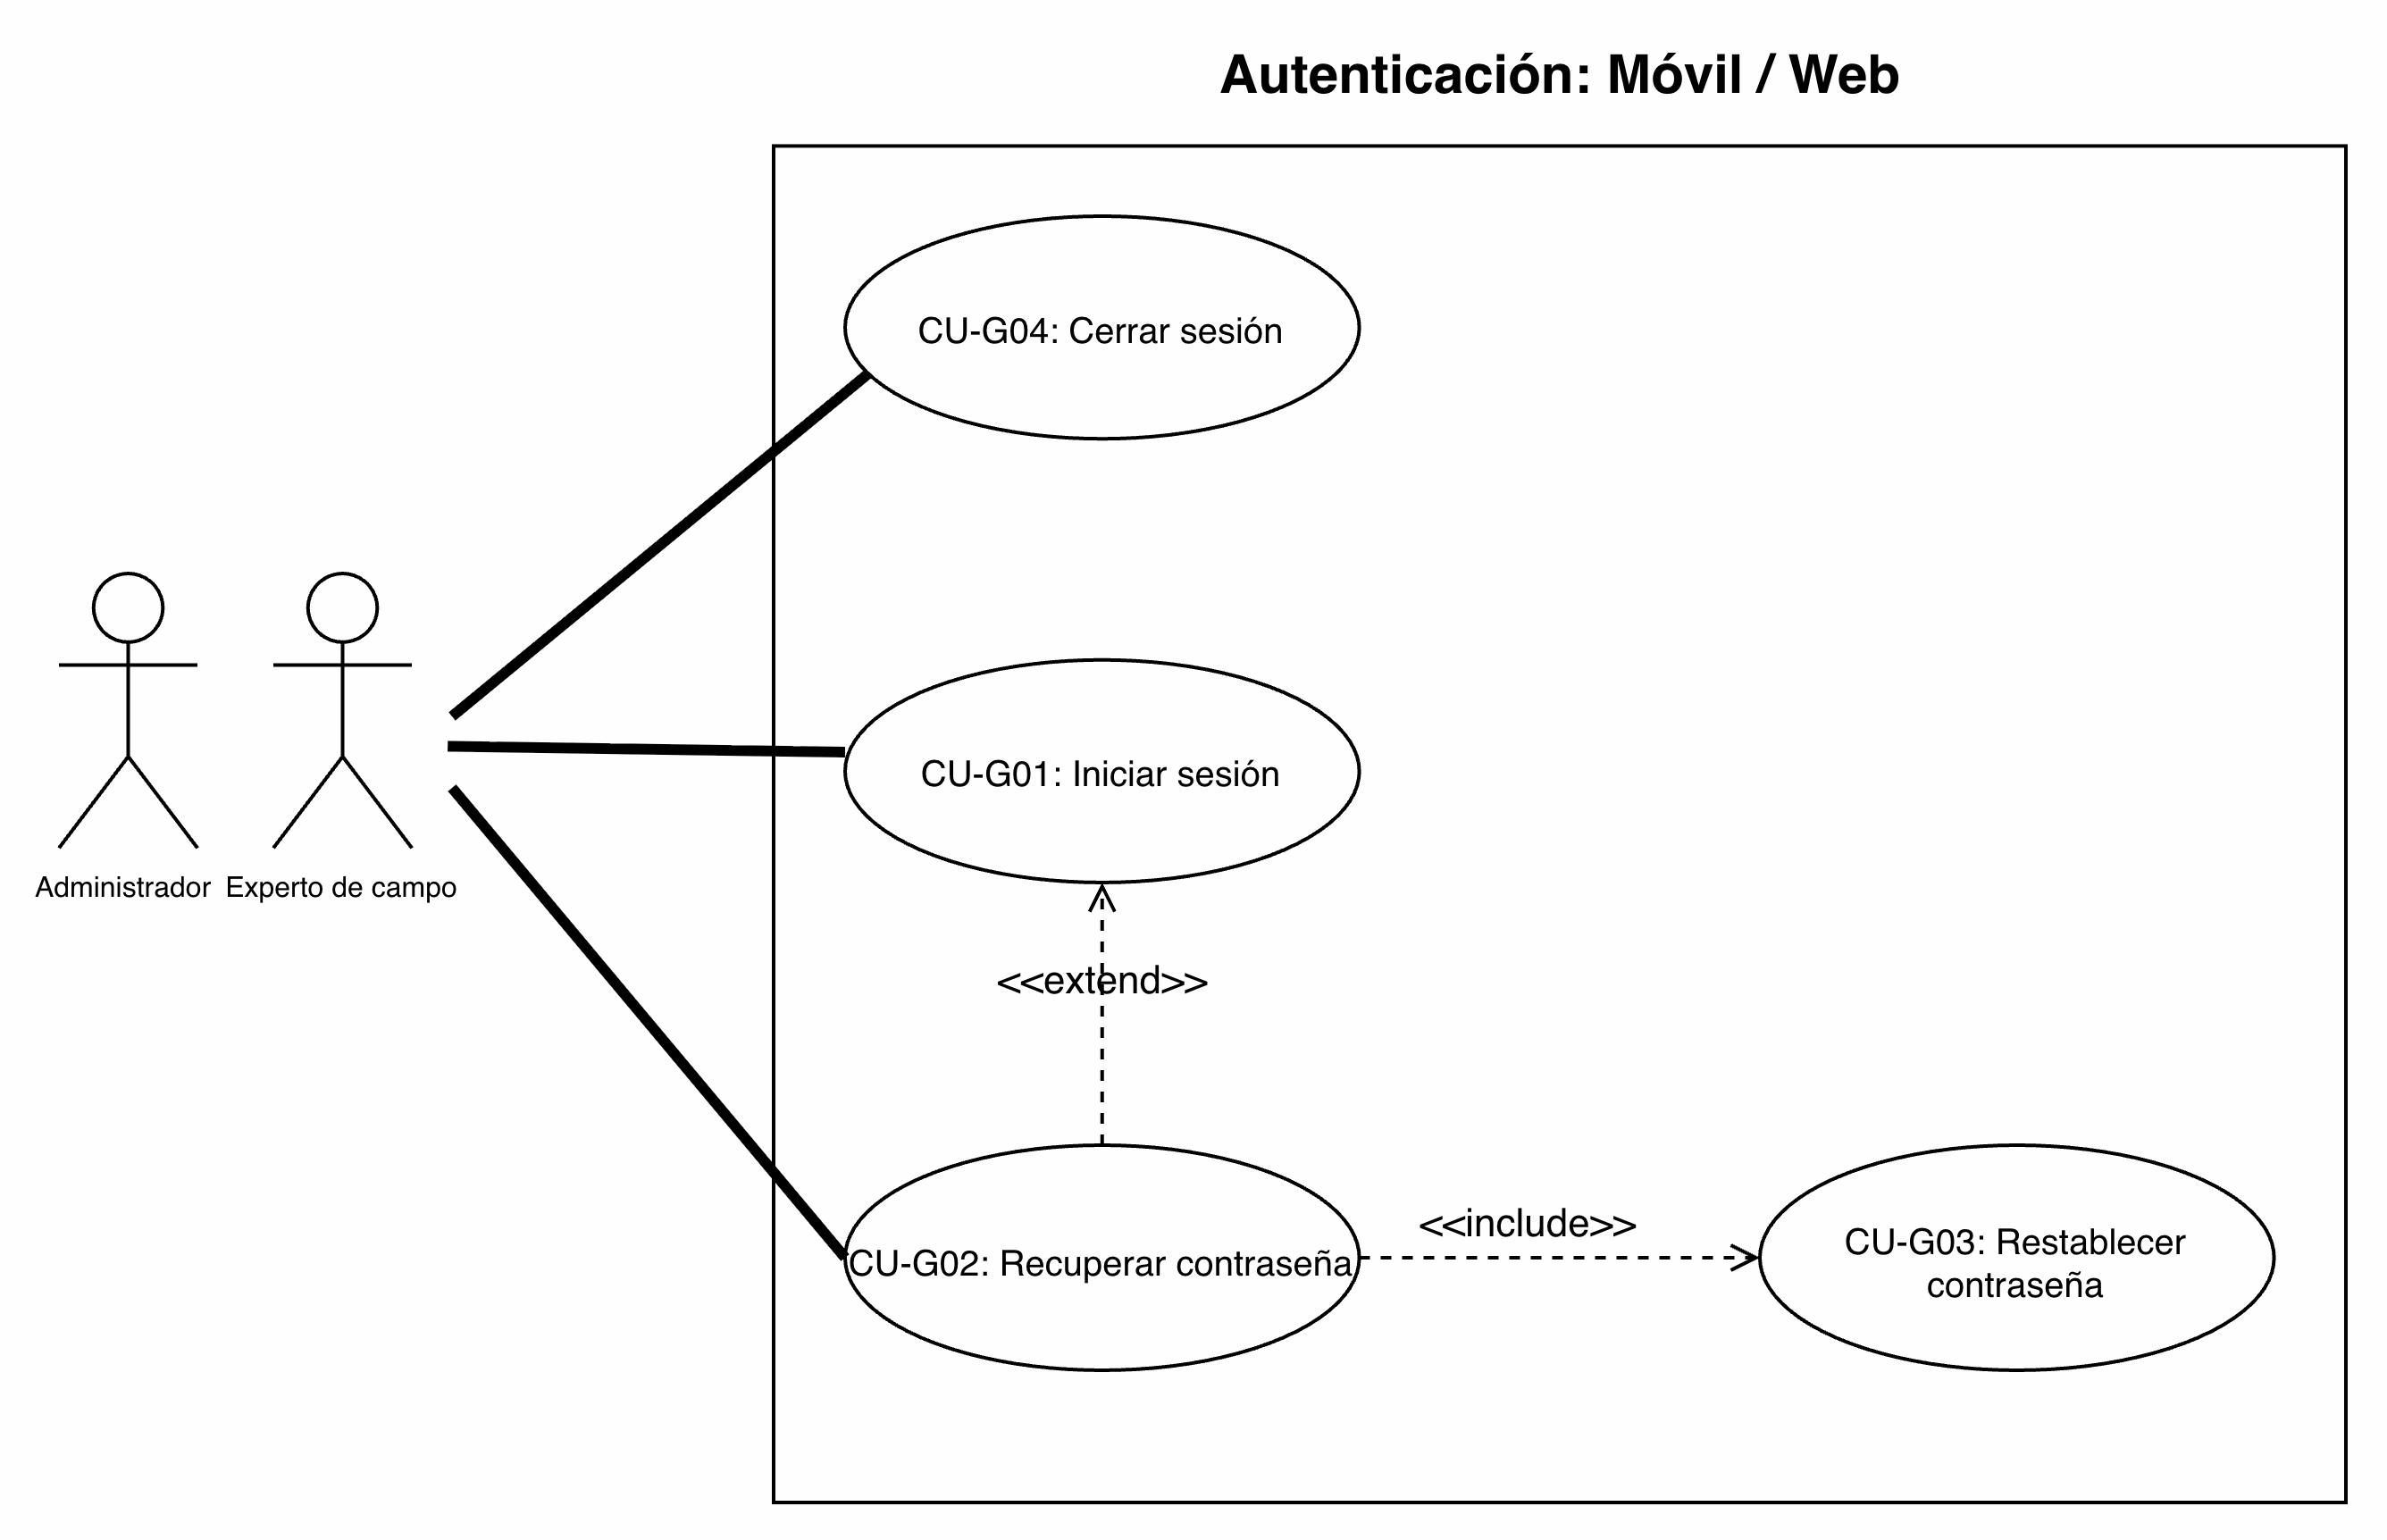
\includegraphics[width=1\textwidth]{images/CU/AUTENTICACION_MOV_WEB.jpeg}
    \caption{CU-G01–CU-G04: Autenticación móvil / web}
\end{figure}

El diagrama representa el flujo general de autenticación del sistema. El Experto de campo puede acceder desde la aplicación móvil y la plataforma web, mientras que el Administrador accede únicamente desde la plataforma web. Ambos actores comparten los casos de uso de iniciar sesión, recuperar contraseña, restablecer contraseña y cerrar sesión. La recuperación de contraseña extiende al inicio de sesión cuando el usuario no recuerda sus credenciales, y el restablecimiento forma parte del proceso de recuperación mediante correo electrónico.

\begin{figure}[H]
    \centering
    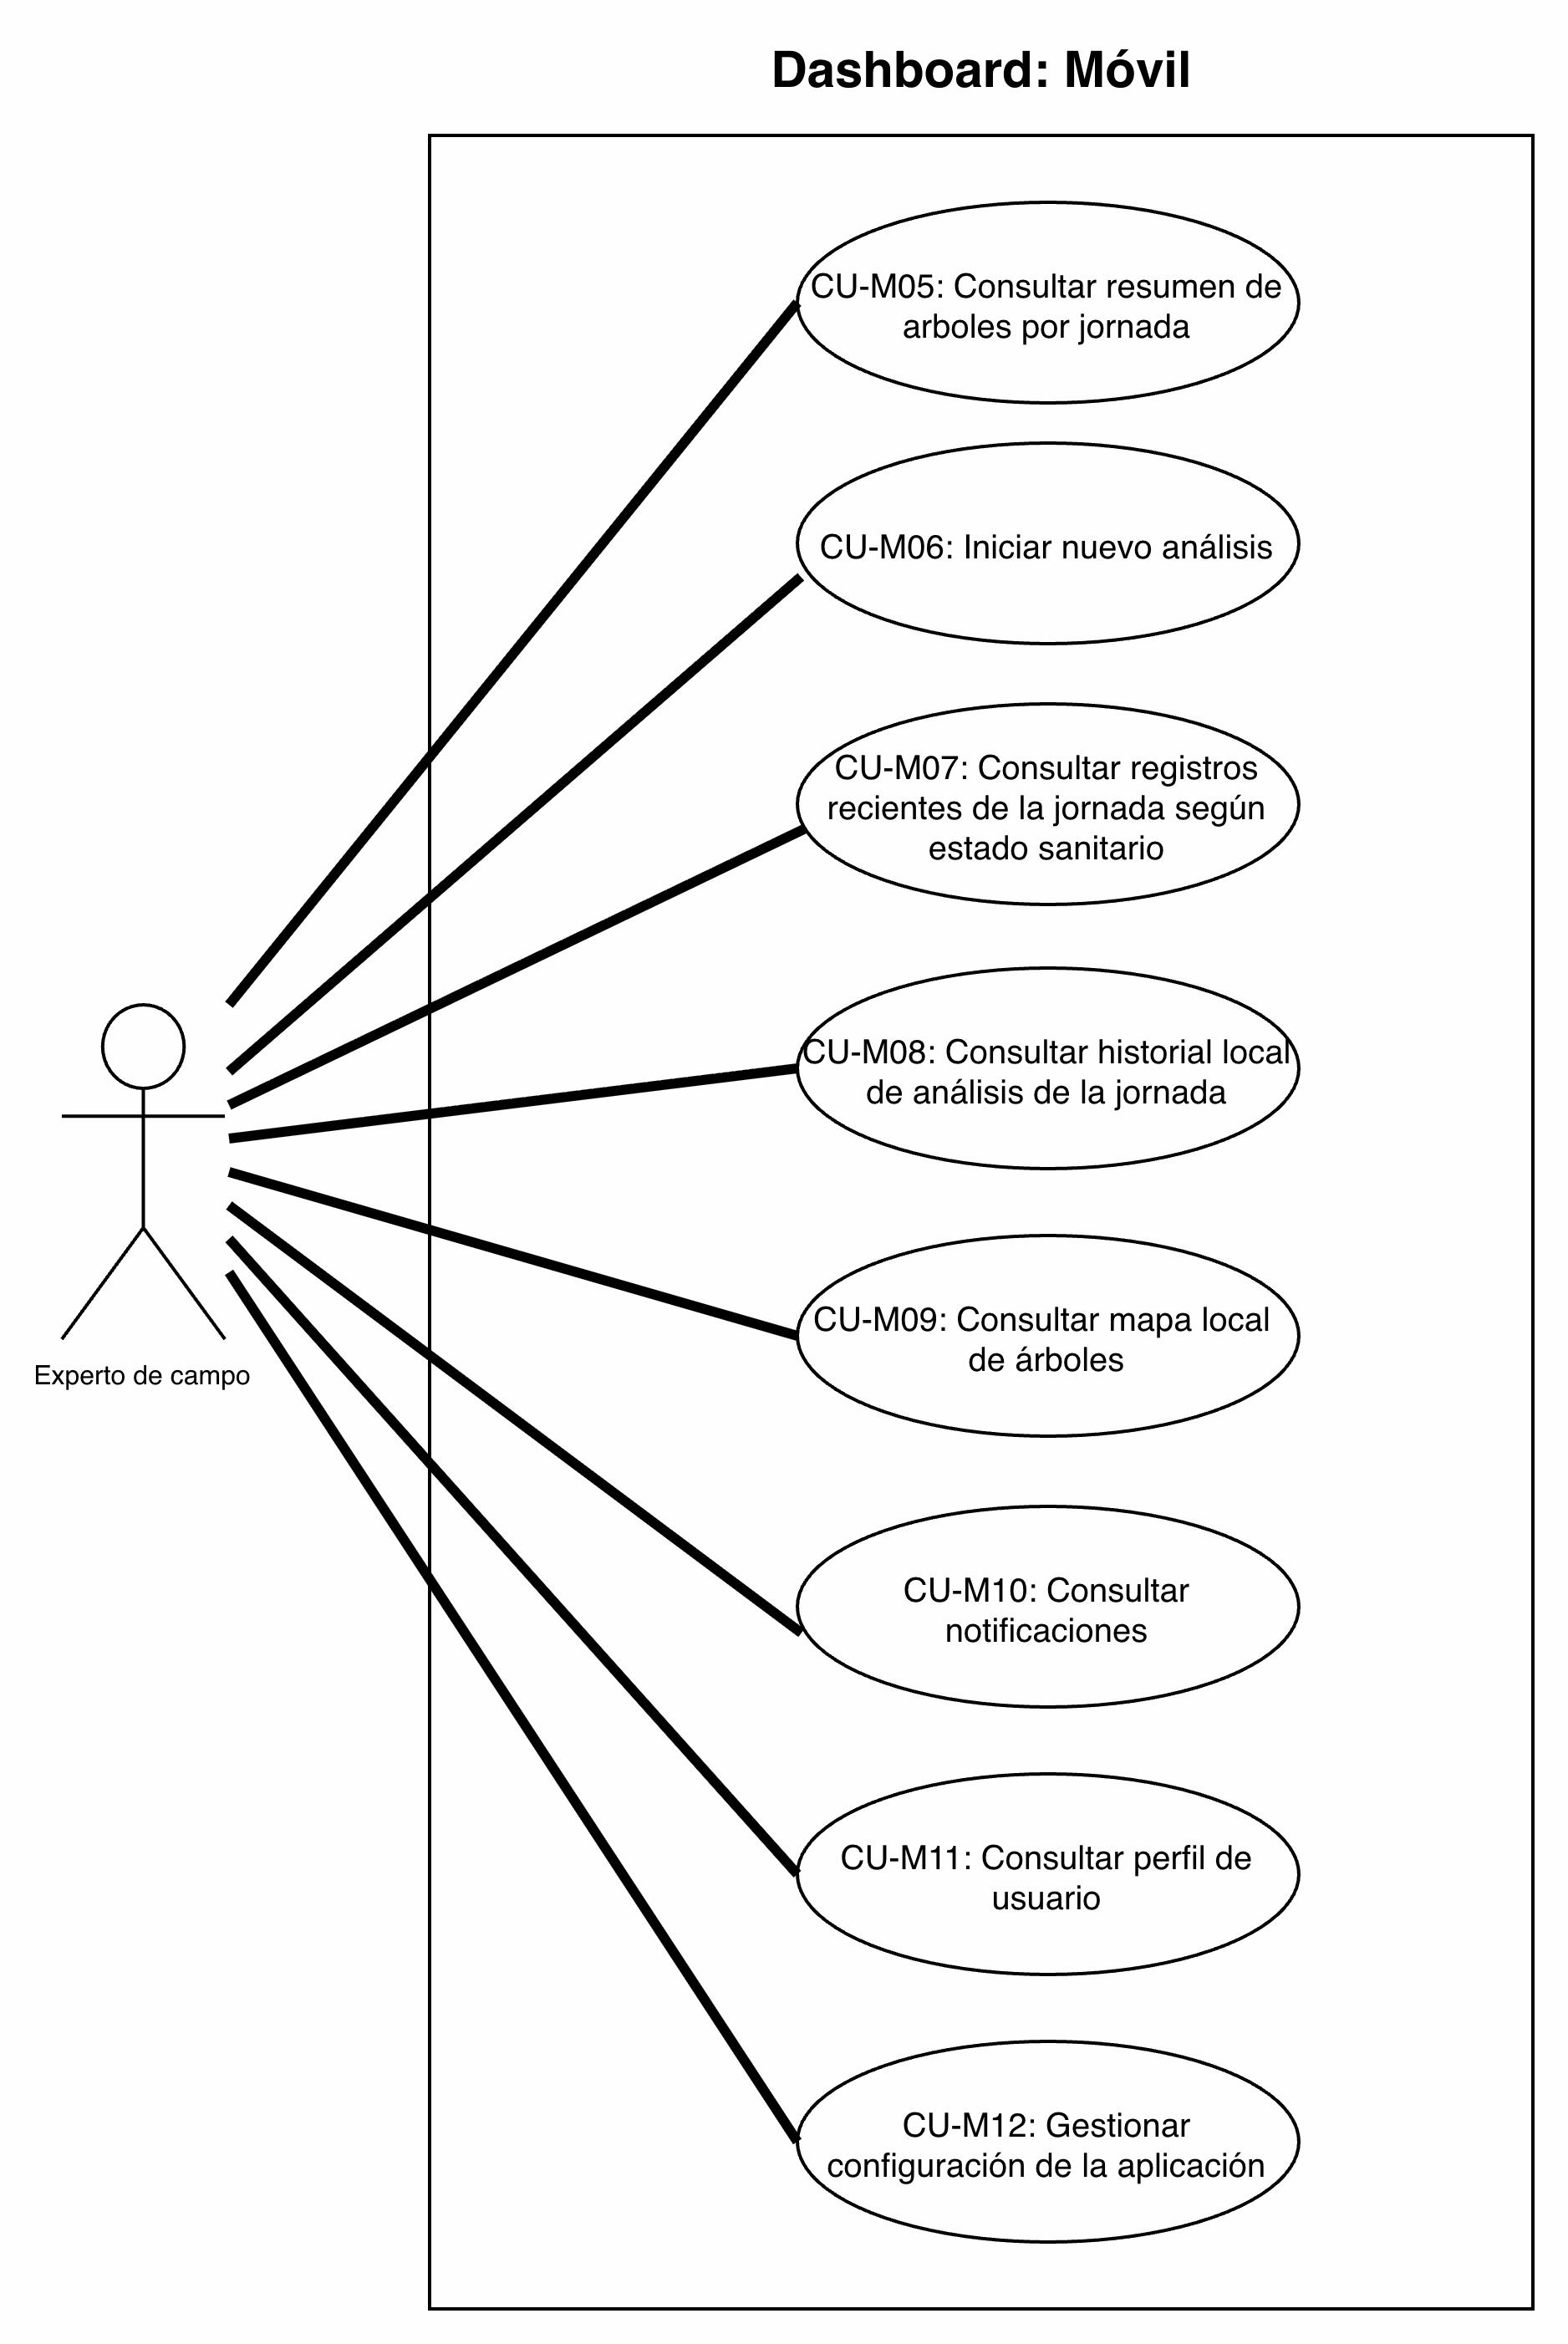
\includegraphics[width=0.8\textwidth]{images/CU/DASH_MOV.jpeg}
    \caption{CU-M05–CU-M12: Dashboard móvil}
\end{figure}

El diagrama muestra las acciones principales disponibles para el Experto de campo desde la pantalla inicial de la aplicación móvil. Desde el dashboard puede consultar el resumen de árboles por jornada, iniciar un nuevo análisis, revisar registros recientes según estado sanitario, consultar el historial local, acceder al mapa local de árboles, revisar notificaciones, consultar su perfil y gestionar la configuración de la aplicación.

\begin{figure}[H]
    \centering
    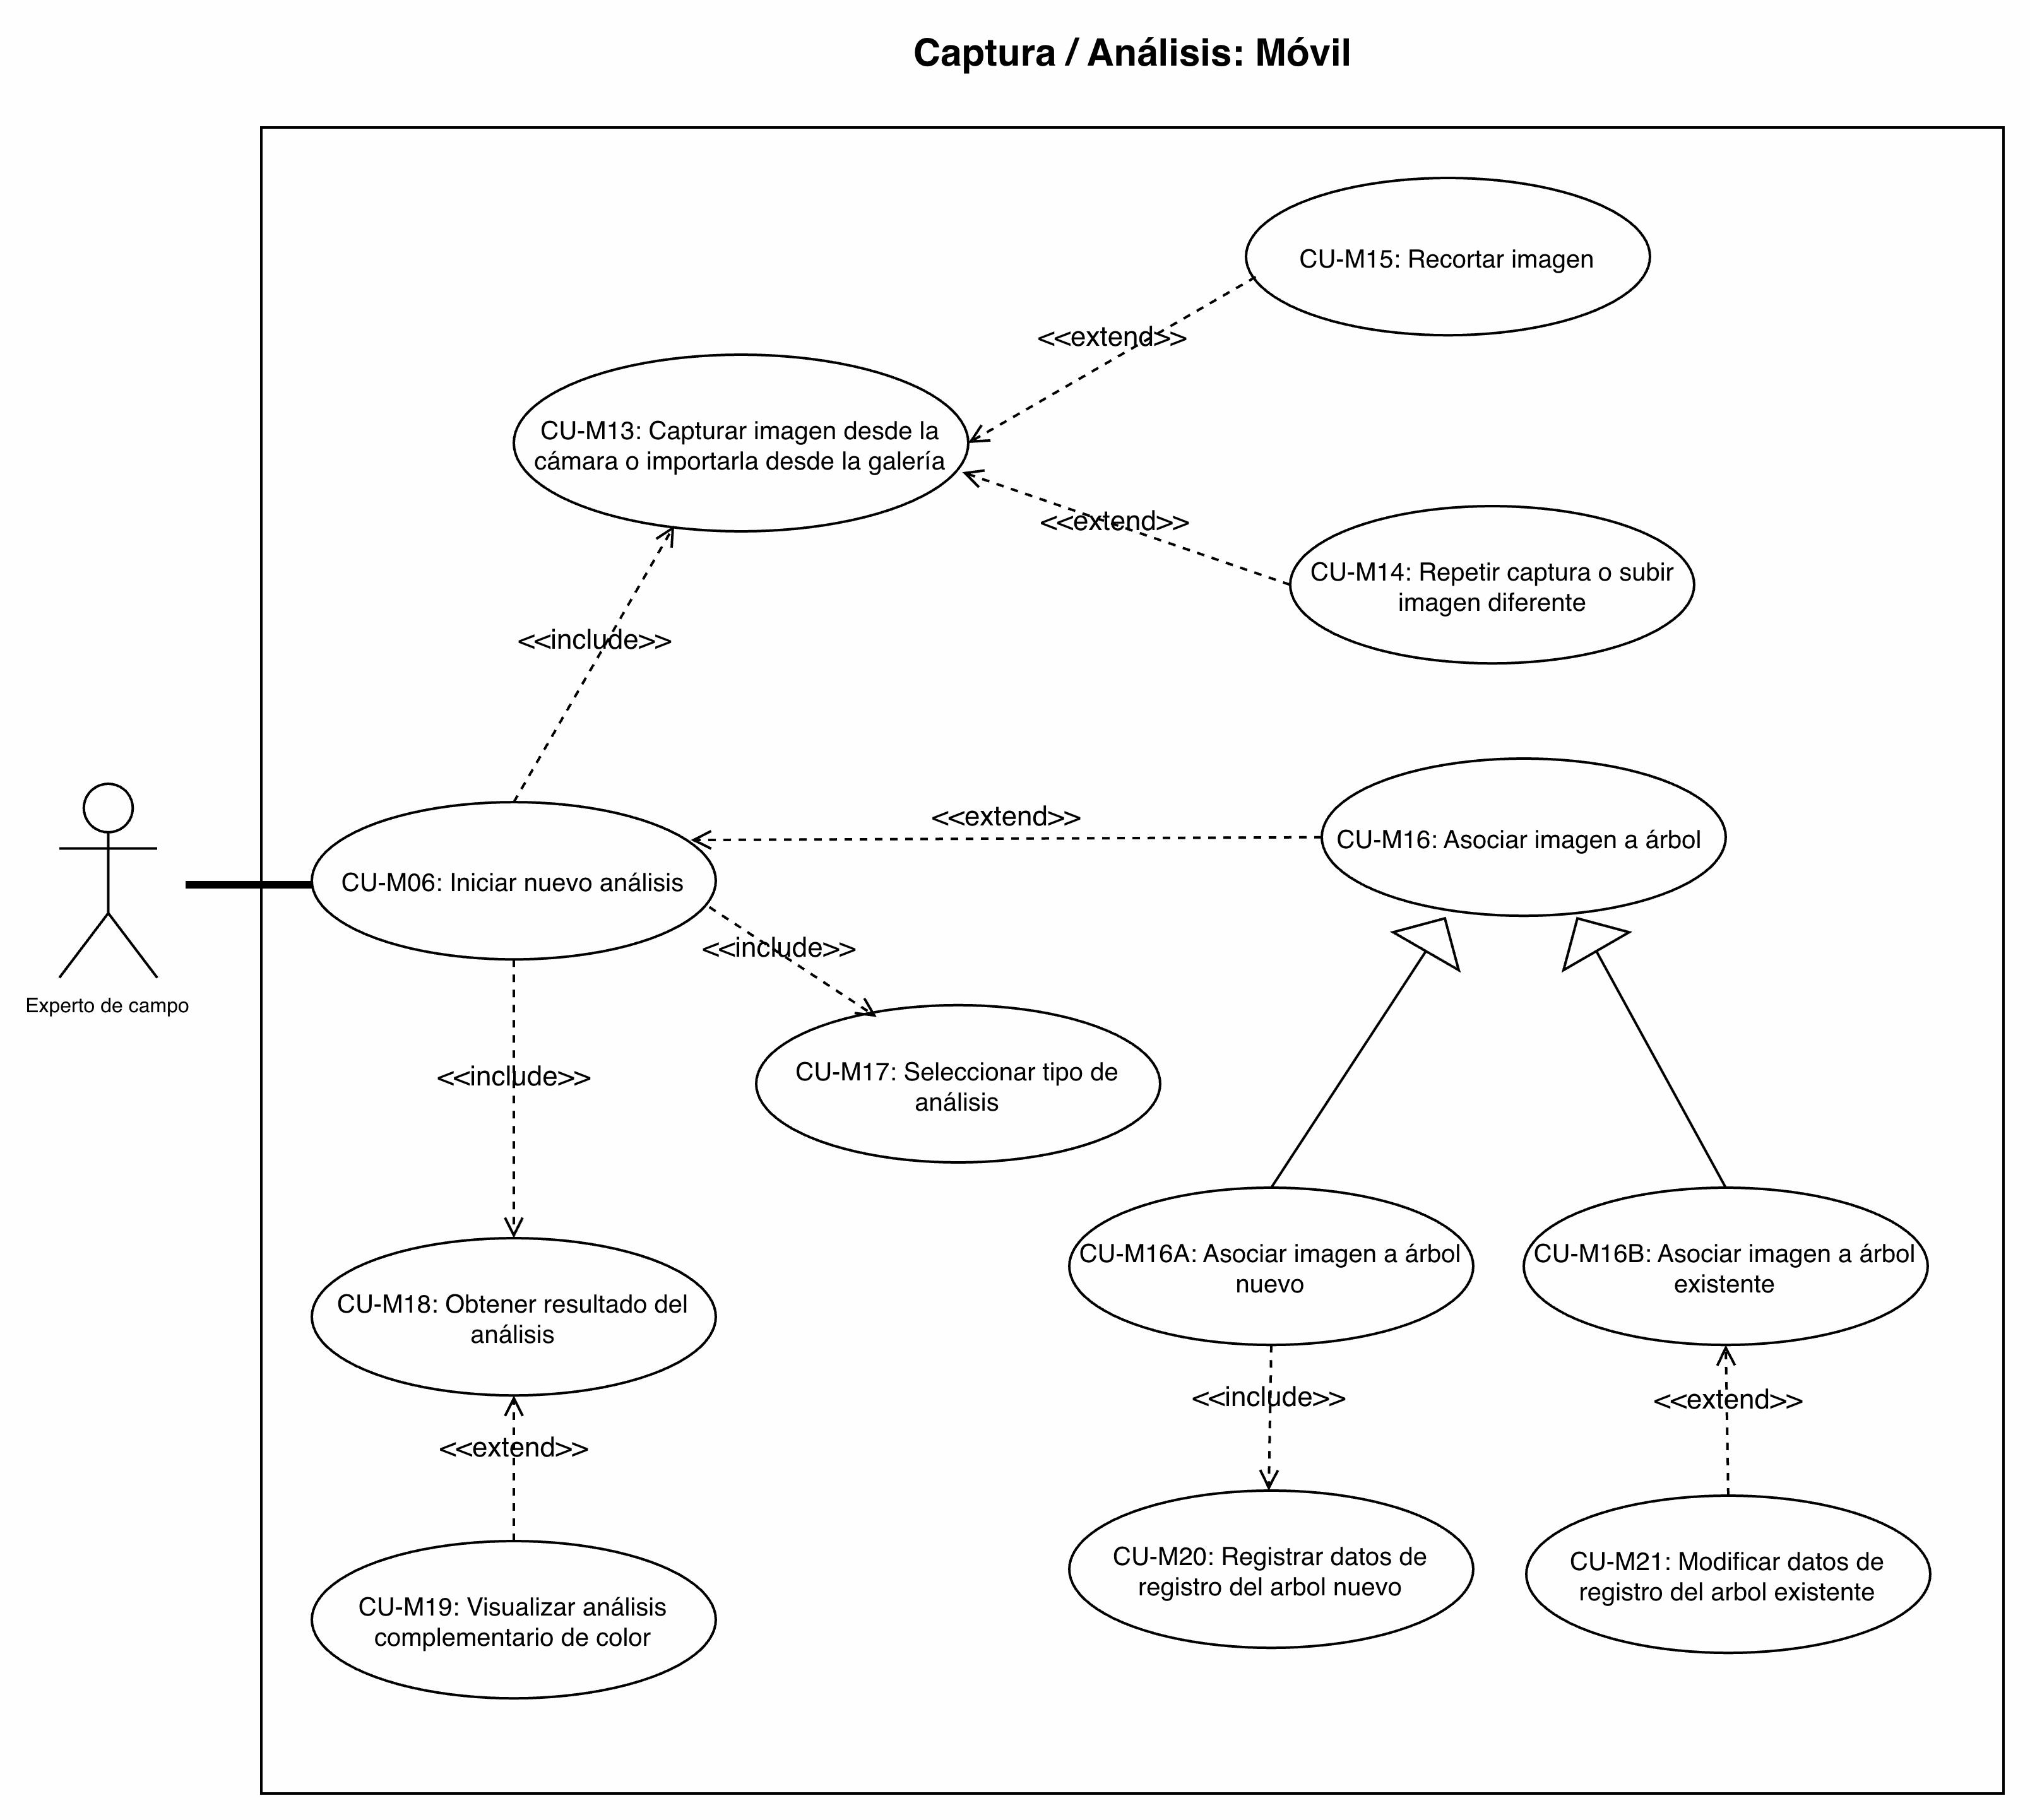
\includegraphics[width=1\textwidth]{images/CU/CAPTURA_MOV.jpeg}
    \caption{CU-M06 y CU-M13–CU-M21: Captura y análisis móvil}
\end{figure}

El diagrama muestra las acciones disponibles para el Experto de campo al iniciar un nuevo análisis desde la aplicación móvil. El usuario puede capturar una imagen desde la cámara o importarla desde la galería, recortarla o repetir la captura si es necesario. La imagen debe asociarse a un árbol, ya sea nuevo o existente. Si el árbol es nuevo, se registran sus datos; si ya existe, sus datos pueden modificarse. El sistema obtiene la clasificación del estado sanitario y, cuando aplica, permite visualizar el análisis complementario de color.

\begin{figure}[H]
    \centering
    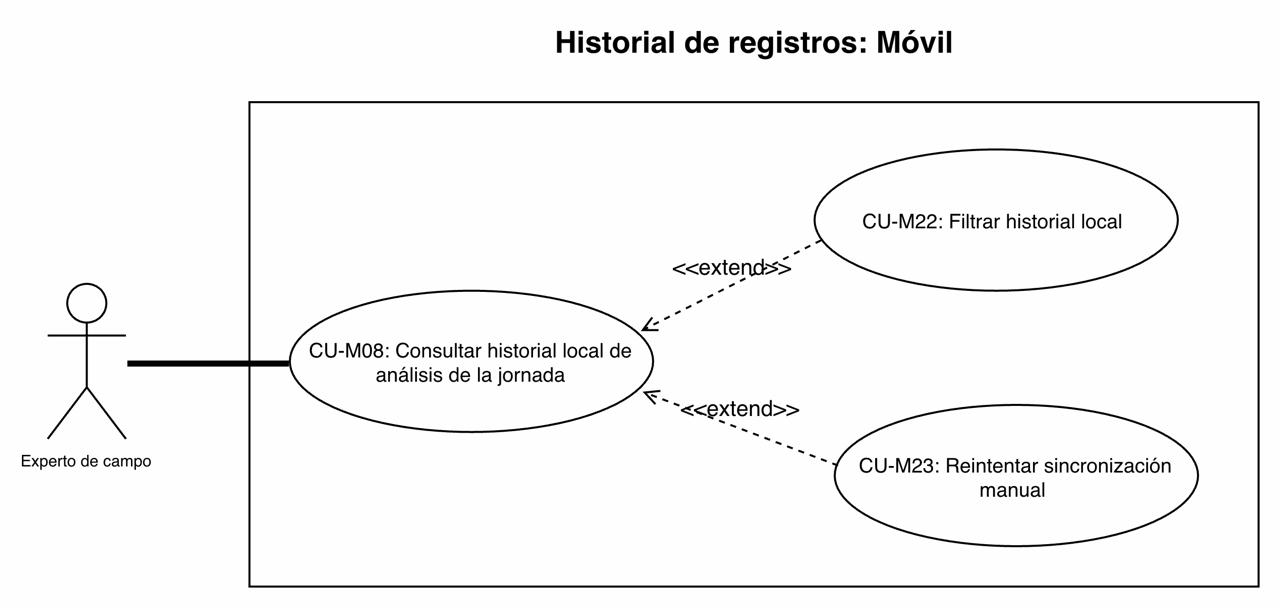
\includegraphics[width=1\textwidth]{images/CU/HISTORIAL_MOV.jpeg}
    \caption{CU-M08 y CU-M22–CU-M23: Historial de registros móvil}
\end{figure}

El diagrama muestra las funciones disponibles en el historial local de la aplicación móvil. El Experto de campo puede consultar los análisis realizados durante la jornada en el dispositivo, filtrar el historial local y reintentar manualmente la sincronización cuando algún registro presente error. El historial móvil utiliza únicamente la base local SQLite del dispositivo en uso.


\begin{figure}[H]
    \centering
    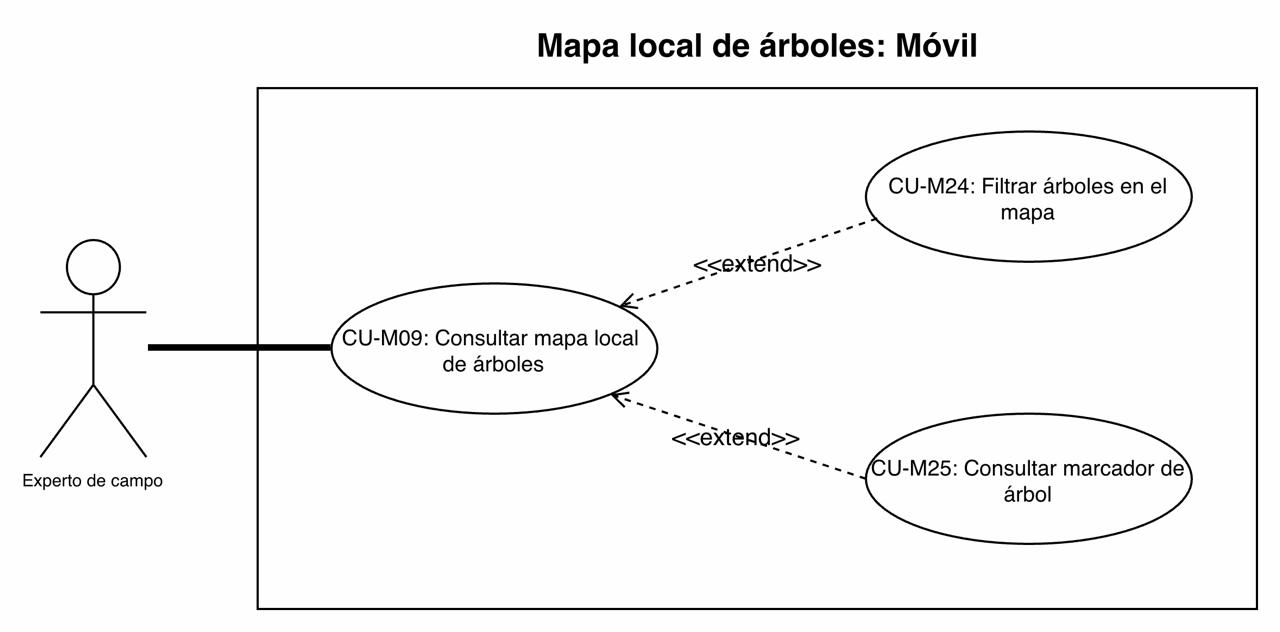
\includegraphics[width=1\textwidth]{images/CU/MAPA_MOV.jpeg}
    \caption{CU-M09 y CU-M24–CU-M25: Mapa local de árboles móvil}
\end{figure}

El diagrama muestra las acciones disponibles en el mapa local de la aplicación móvil. El Experto de campo puede consultar los árboles registrados en el dispositivo, aplicar filtros en el mapa y revisar la información de un marcador seleccionado. La información mostrada corresponde únicamente a los registros almacenados en la base local SQLite del dispositivo móvil en uso.

\begin{figure}[H]
    \centering
    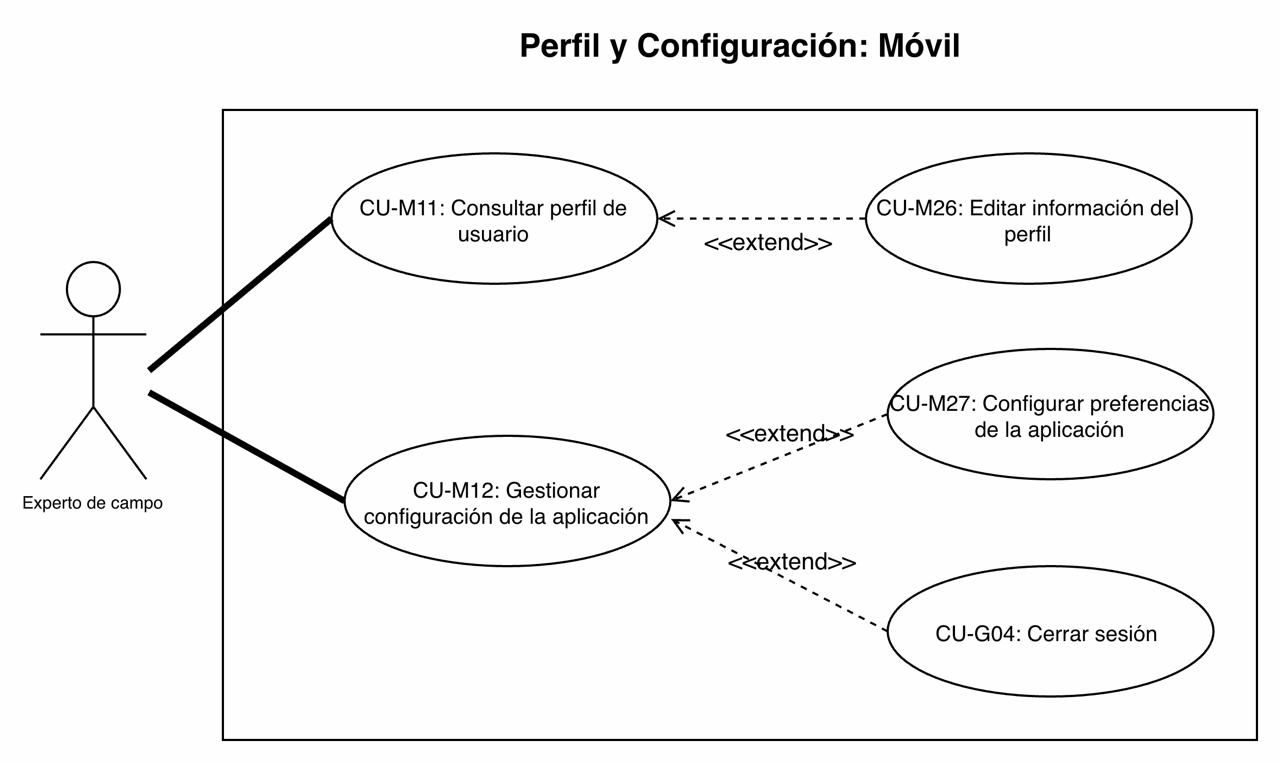
\includegraphics[width=1\textwidth]{images/CU/PERFIL_CONF_MOV.jpeg}
    \caption{CU-M11–CU-M12 y CU-M26–CU-M27, CU-G04: Perfil y configuración móvil}
\end{figure}

El diagrama muestra las funciones disponibles para el Experto de campo dentro del perfil y configuración de la aplicación móvil. Desde esta sección puede consultar y editar información de su perfil, gestionar la configuración de la aplicación, configurar preferencias y cerrar sesión. El cierre de sesión reutiliza el caso de uso general de autenticación.

\begin{figure}[H]
    \centering
    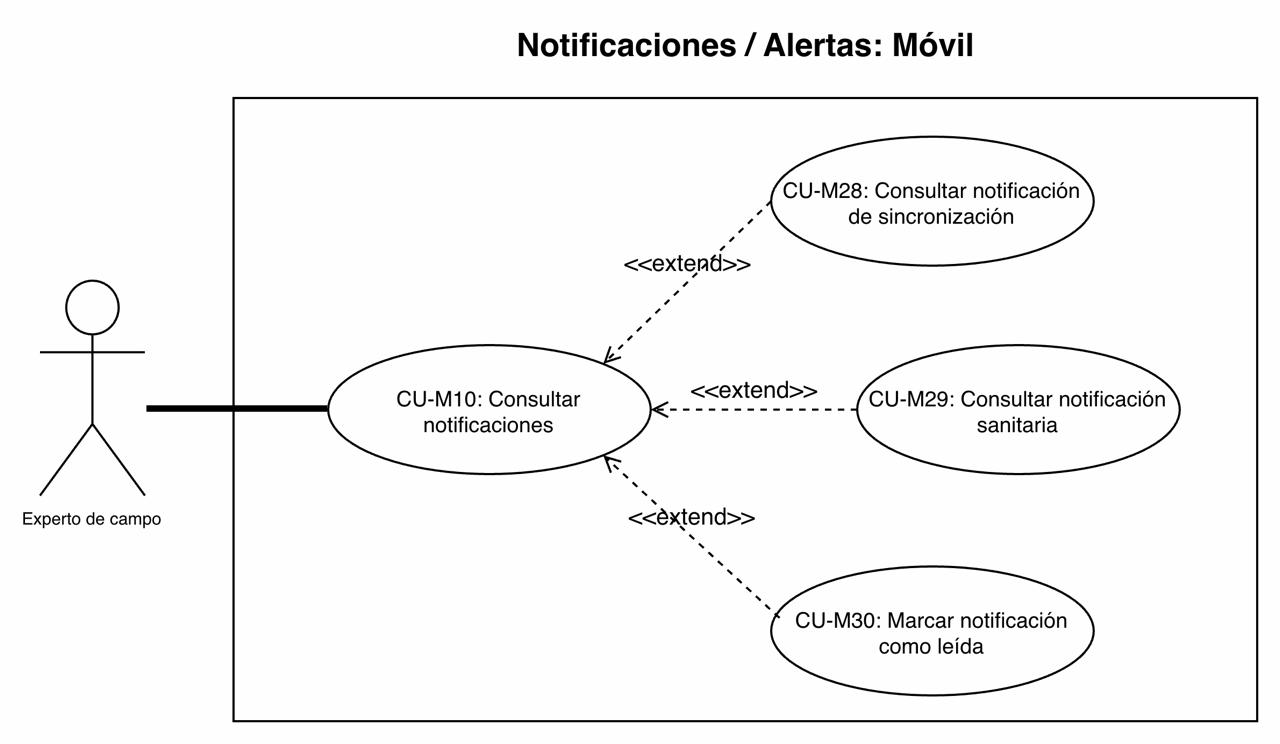
\includegraphics[width=1\textwidth]{images/CU/NOTIS_MOV.jpeg}
    \caption{CU-M10 y CU-M28–CU-M30: Notificaciones y alertas móvil}
\end{figure}

El diagrama muestra las acciones disponibles en la sección de notificaciones de la aplicación móvil. El Experto de campo puede consultar notificaciones generales, revisar notificaciones de sincronización, consultar notificaciones sanitarias y marcar notificaciones como leídas. Las notificaciones de sincronización informan sobre registros pendientes, sincronizados o con error, mientras que las sanitarias alertan sobre resultados relevantes del análisis o posibles riesgos asociados al estado sanitario de los árboles.

\begin{figure}[H]
    \centering
    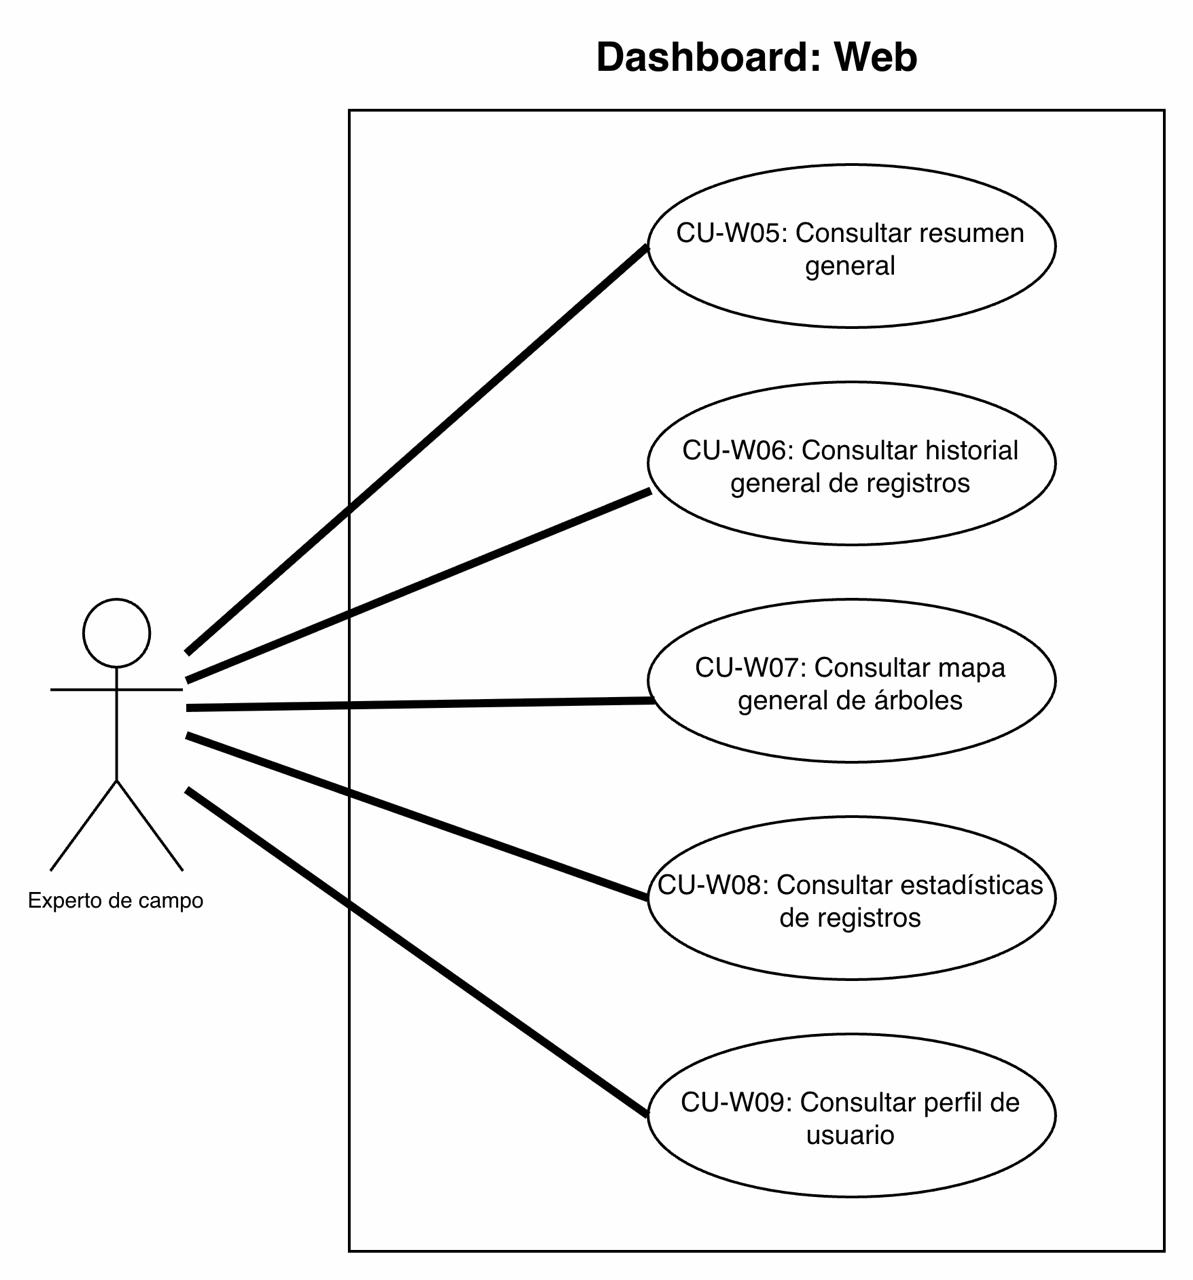
\includegraphics[width=1\textwidth]{images/CU/DASH_WEB.jpeg}
    \caption{CU-W05–CU-W09: Dashboard web}
\end{figure}

El diagrama representa las acciones principales disponibles para el Experto de campo desde el dashboard de la plataforma web. A diferencia del dashboard móvil, esta vista consulta información consolidada en la nube. Desde ella, el usuario puede consultar el resumen general, acceder al historial general de registros, visualizar el mapa general de árboles, revisar estadísticas y consultar su perfil.

\begin{figure}[H]
    \centering
    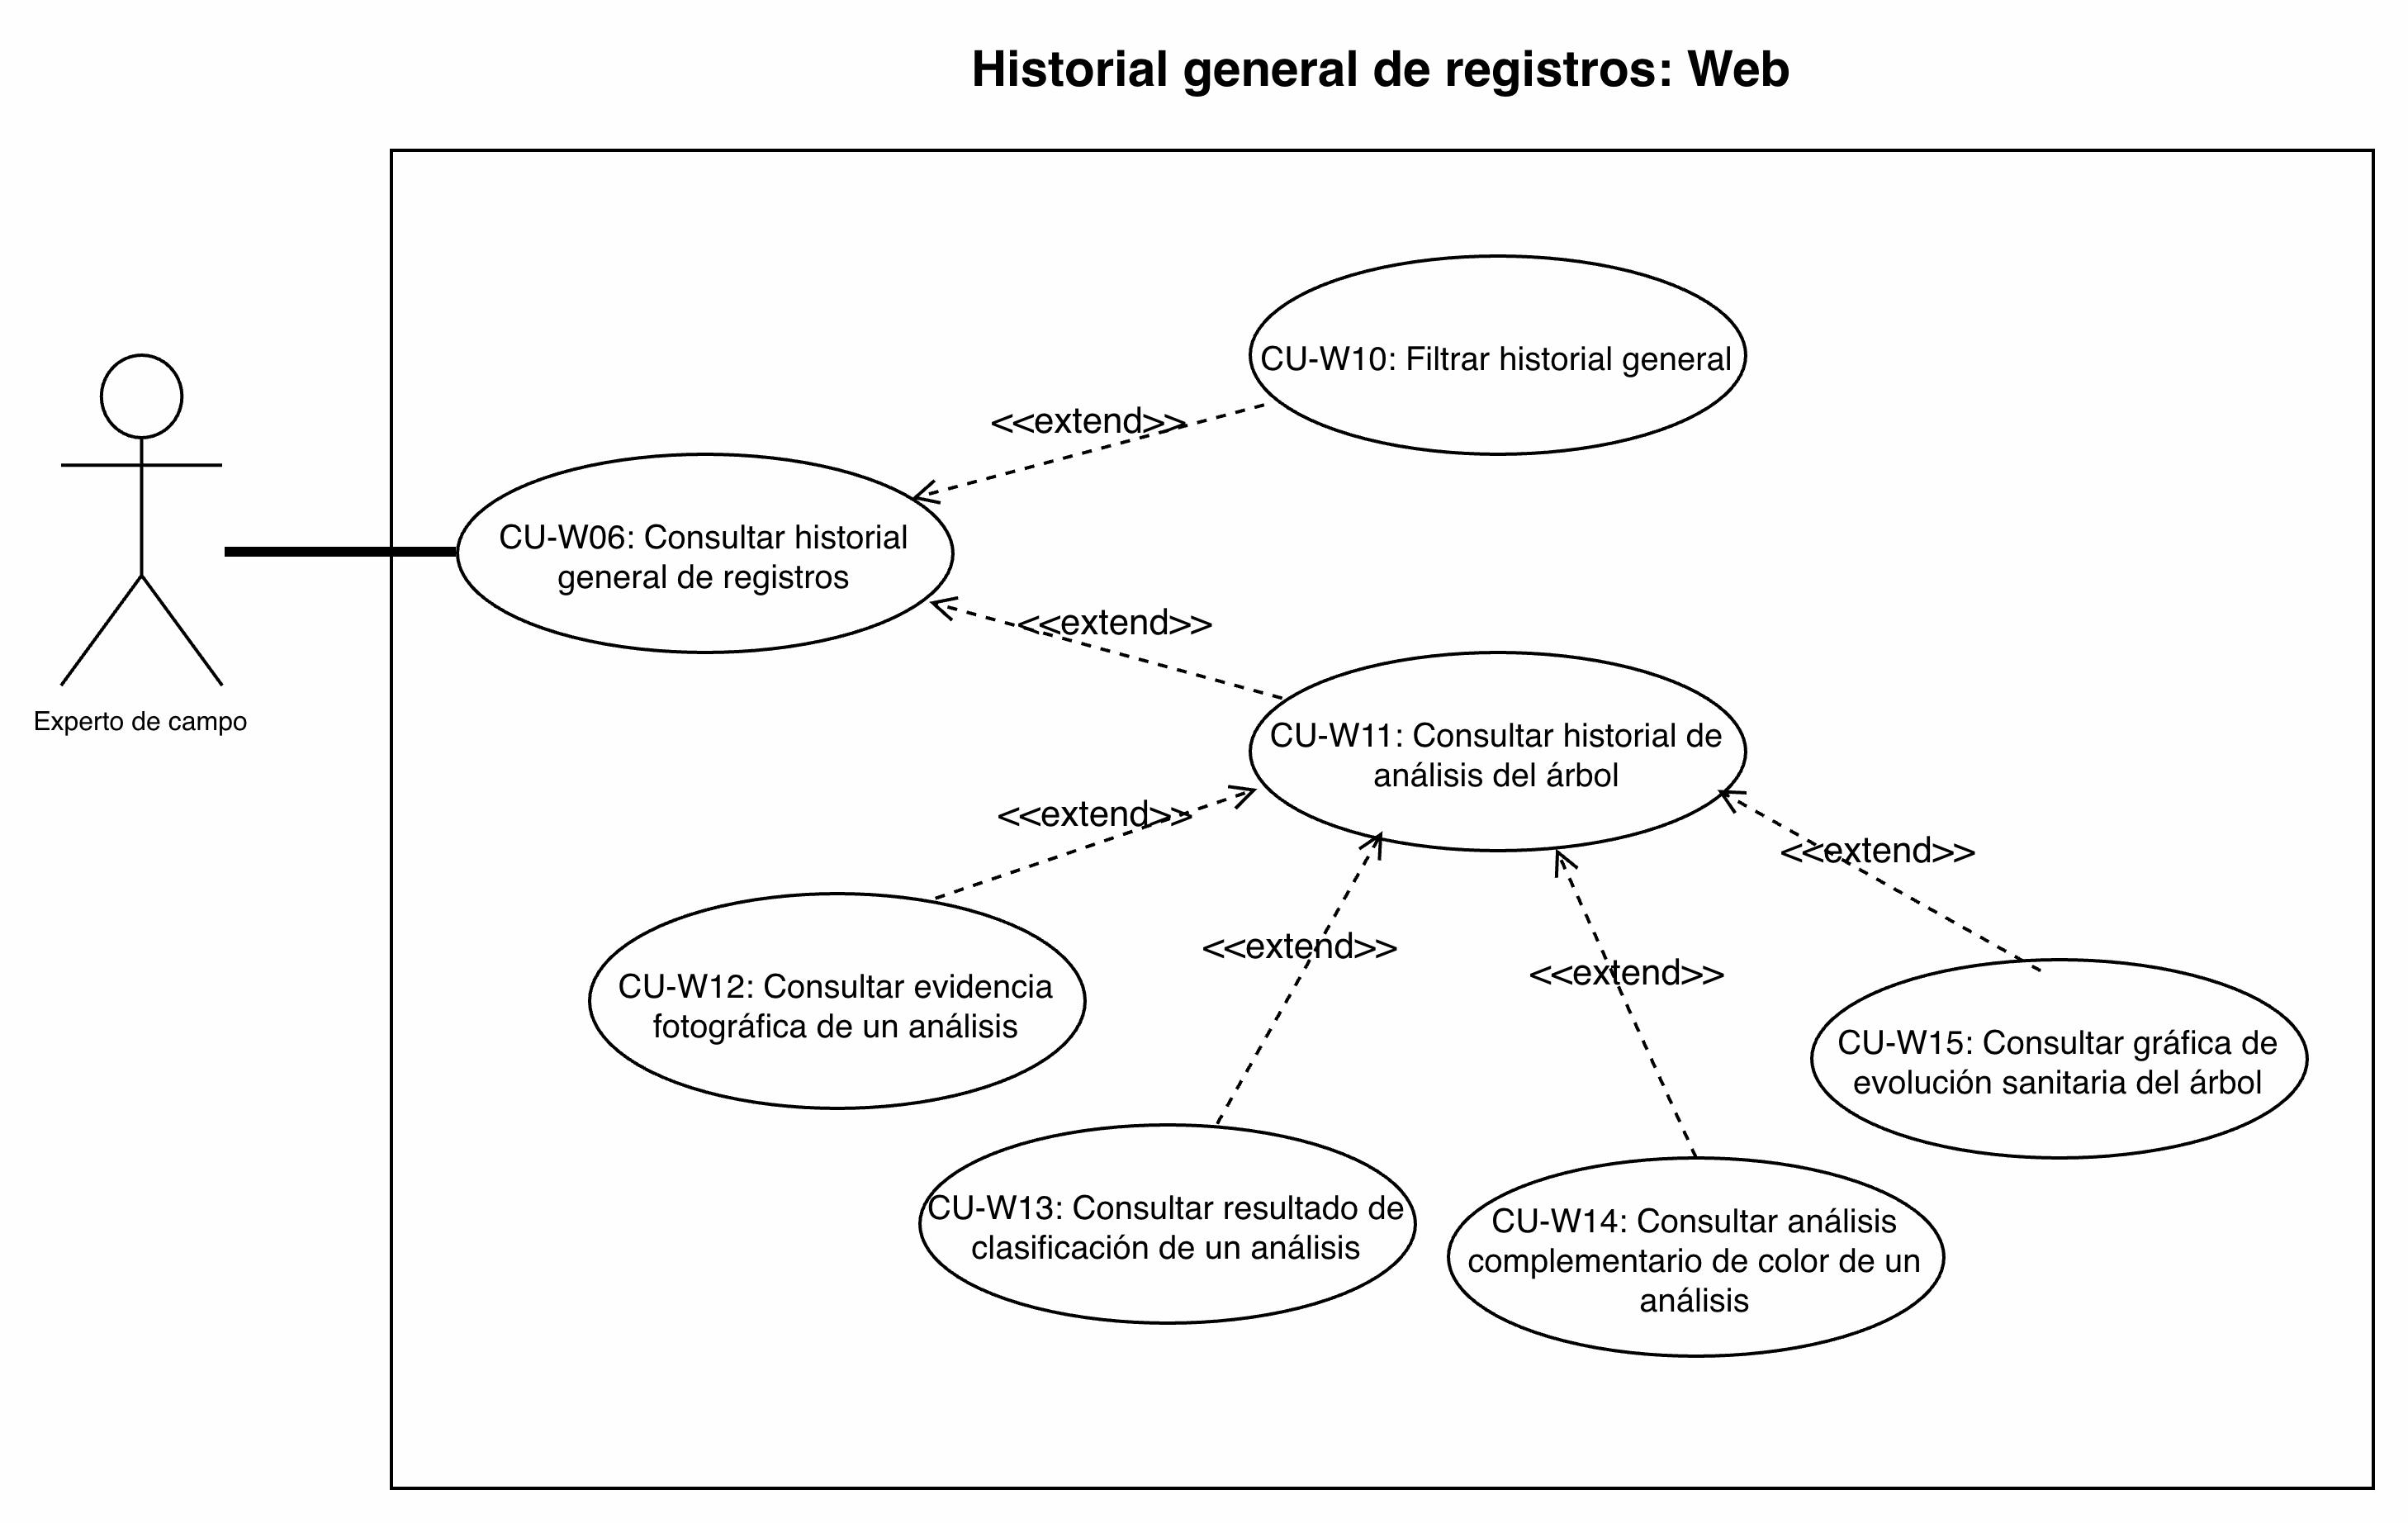
\includegraphics[width=1\textwidth]{images/CU/HISTORIAL_WEB.jpeg}
    \caption{CU-W06 y CU-W10–CU-W15: Historial general de registros web}
\end{figure}

El diagrama representa la consulta del historial general de registros desde la plataforma web. El Experto de campo puede consultar los registros sincronizados en la nube, aplicar filtros generales y acceder al historial de análisis de un árbol. Desde dicho historial puede consultar la evidencia fotográfica, el resultado de clasificación, el análisis complementario de color y la gráfica de evolución sanitaria del árbol. La plataforma web funciona como una vista consolidada de consulta, sin edición de registros operativos.

\begin{figure}[H]
    \centering
    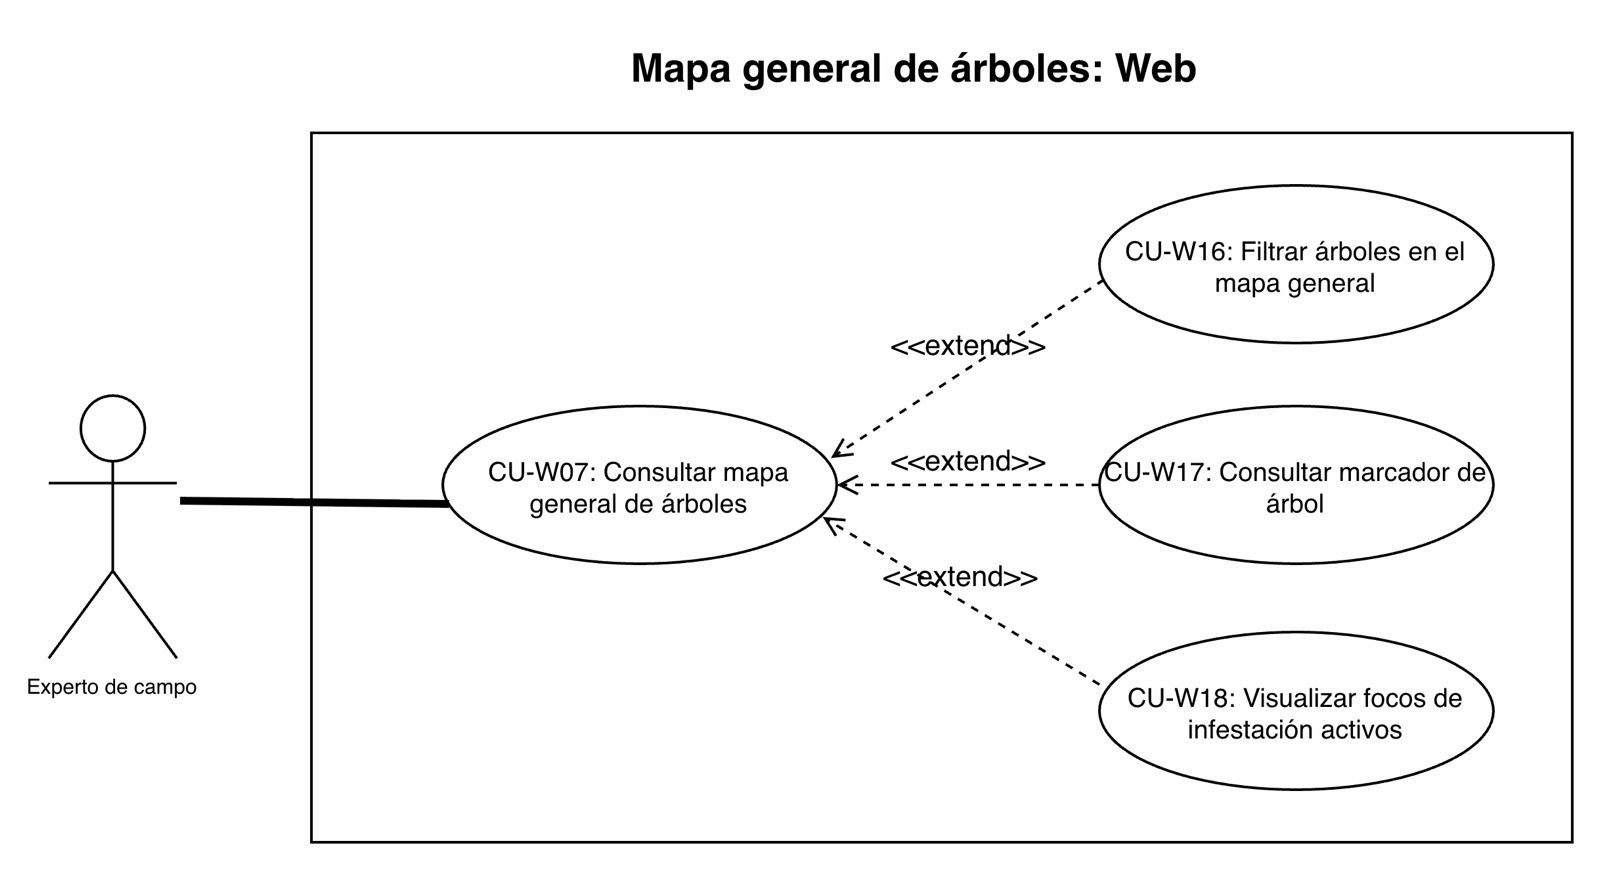
\includegraphics[width=1\textwidth]{images/CU/MAPA_WEB.jpeg}
    \caption{CU-W07 y CU-W16–CU-W18: Mapa general de árboles web}
\end{figure}

El diagrama representa la consulta del mapa general de árboles desde la plataforma web. El Experto de campo puede visualizar los árboles sincronizados desde todos los dispositivos asociados a su cuenta, aplicar filtros sobre el mapa, consultar marcadores específicos y visualizar focos de infestación activos generados a partir de los registros consolidados en la nube.

\begin{figure}[H]
    \centering
    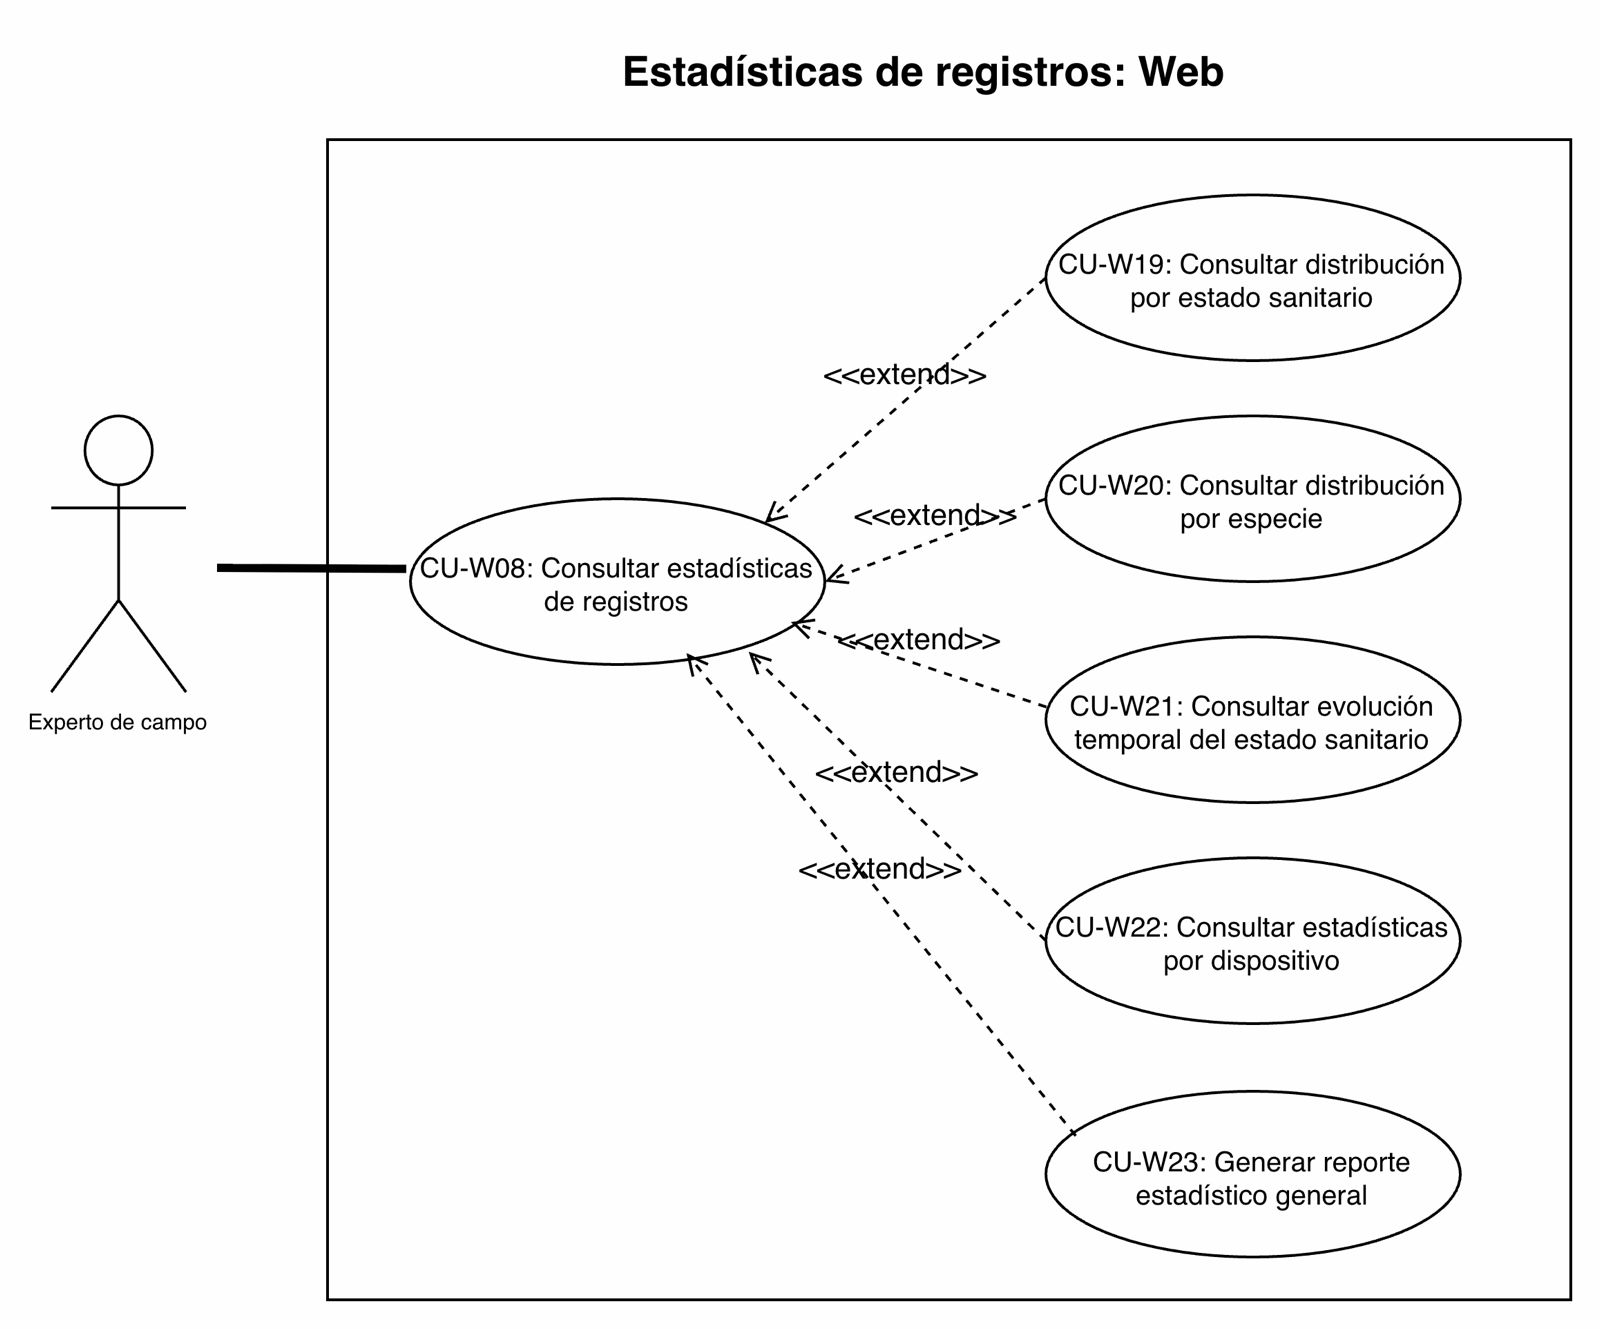
\includegraphics[width=1\textwidth]{images/CU/ESTADISTICAS_WEB.jpeg}
    \caption{CU-W08 y CU-W19–CU-W23: Estadísticas de registros web}
\end{figure}

El diagrama muestra las funciones estadísticas disponibles para el Experto de campo en la plataforma web. El usuario puede consultar estadísticas generadas a partir de los registros sincronizados en la nube, incluyendo distribución por estado sanitario, distribución por especie, evolución temporal del estado sanitario y estadísticas por dispositivo de origen. Esta sección es únicamente de consulta y no modifica los registros almacenados.

\begin{figure}[H]
    \centering
    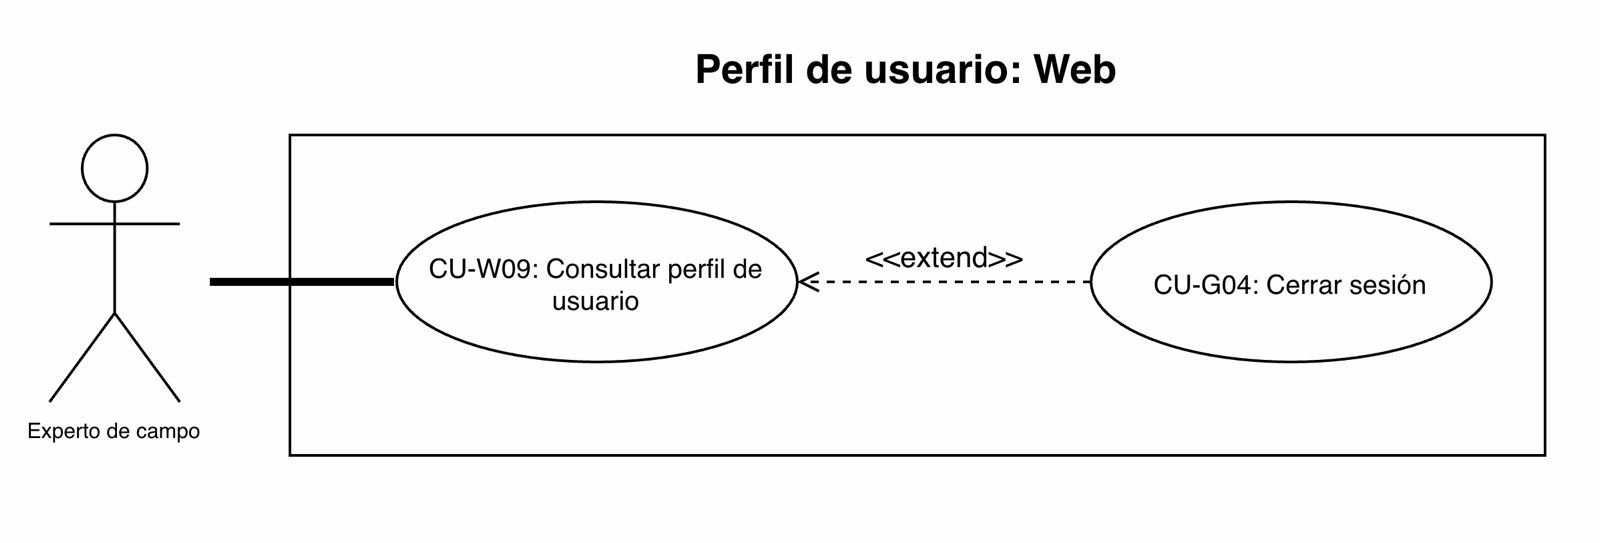
\includegraphics[width=1\textwidth]{images/CU/PERFIL_WEB.jpeg}
    \caption{CU-W09 y CU-G04: Perfil de usuario web}
\end{figure}

El diagrama representa la consulta del perfil de usuario desde la plataforma web. El Experto de campo puede consultar la información de su cuenta y cerrar sesión. No se contemplan acciones de edición desde esta sección, ya que la plataforma web se mantiene como una vista de consulta y supervisión.

\begin{figure}[H]
    \centering
    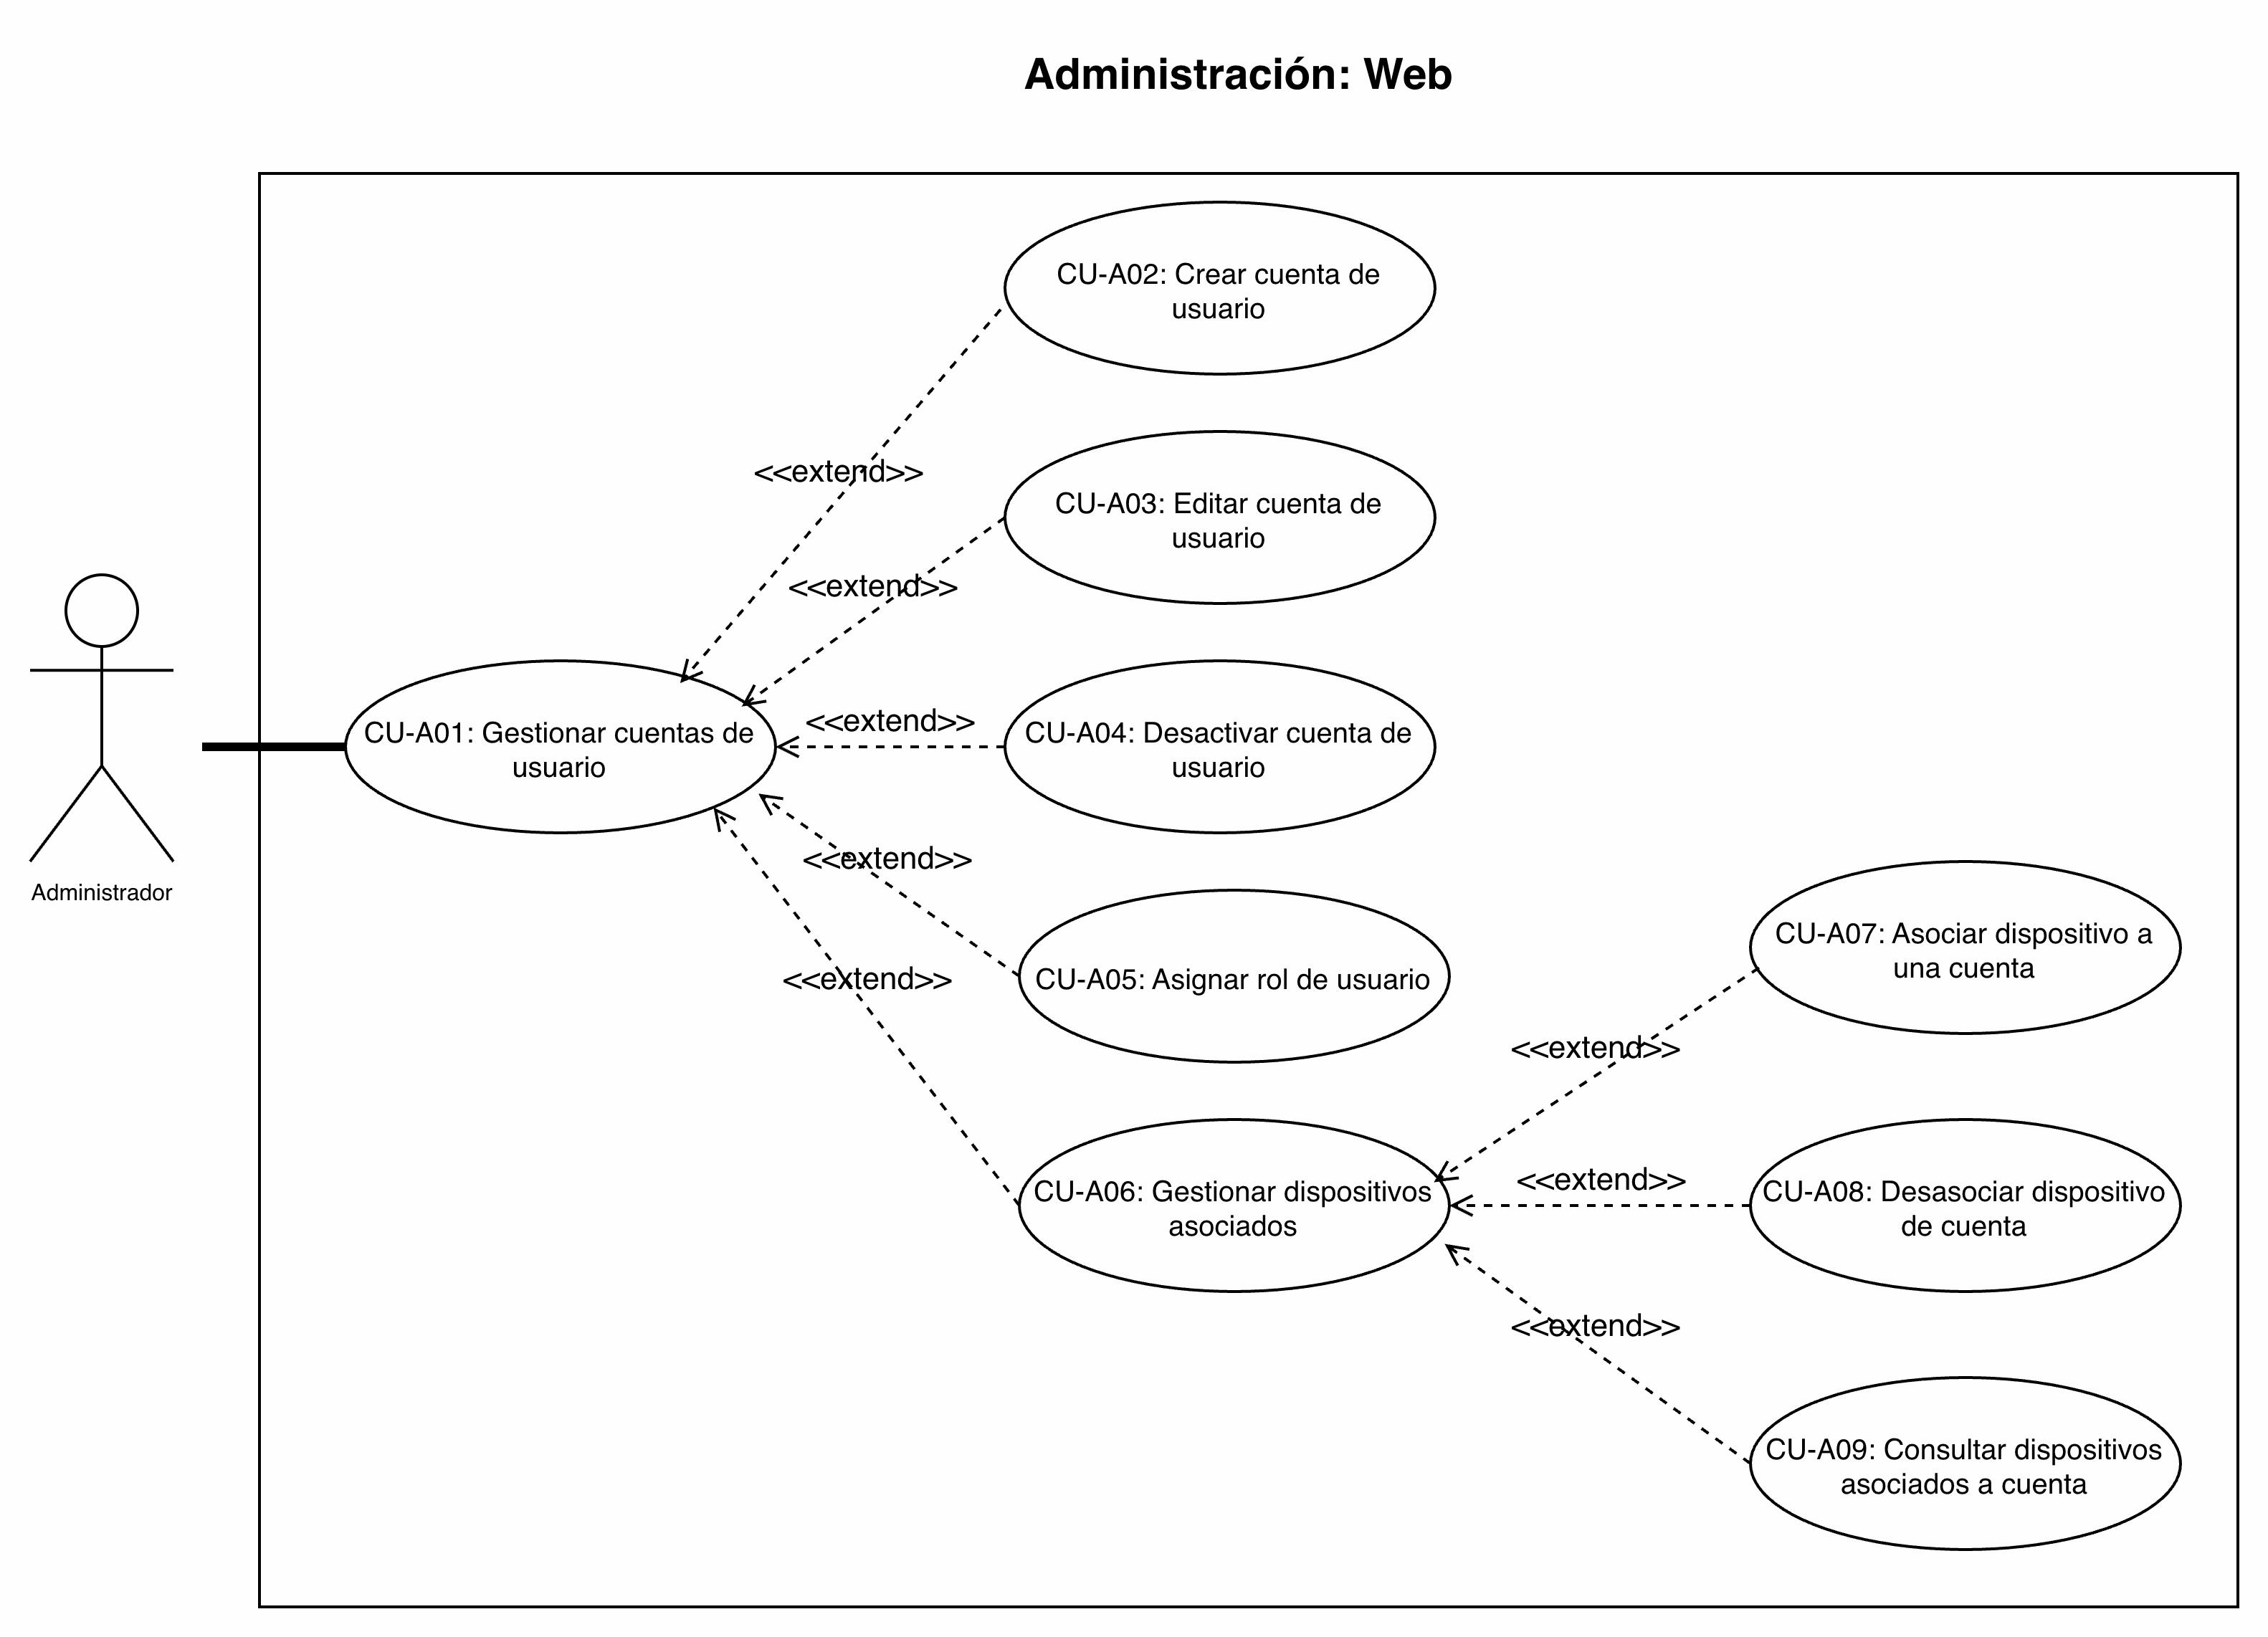
\includegraphics[width=1\textwidth]{images/CU/ADMIN_WEB.jpeg}
    \caption{CU-A01–CU-A09: Administración web}
\end{figure}

El diagrama muestra las funciones disponibles para el Administrador dentro de la plataforma web. Desde este módulo puede gestionar cuentas de usuario, crear, editar o desactivar cuentas, asignar roles y administrar los dispositivos asociados a cada cuenta. La gestión de dispositivos permite consultar, asociar o desasociar dispositivos móviles autorizados para operar con una cuenta de experto.

